\section{Interpreter}

De acordo com GoF, o Interpreter define uma representação para 
a gramática de uma linguagem e usa um interpretador para 
interpretar sentenças dessa linguagem.

Apesar da definição parecer específica, o padrão pode ser 
generalizado para qualquer hierarquia de classes, desde que 
não seja muito complexa. Dessa forma, o padrão permite 
interpretar essa hierarquia e realizar uma operação que 
dependa da forma como essas classes estão dispostas, por 
exemplo.

\begin{figure}[htb]
	\caption{\label{fig_grafico}Estrutura do Interpreter}
	\begin{center}
	    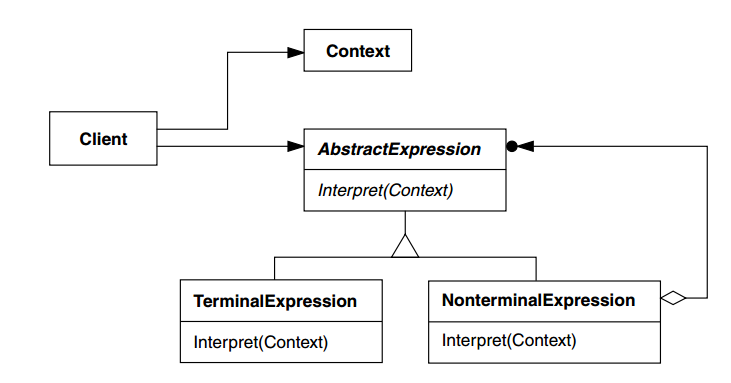
\includegraphics[scale=0.5]{5_padroes-contexto-funcional/5.3_comportamentais/5.3.03_interpreter/diagram.png}
	\end{center}
\end{figure}

Exemplo Orientado a Objetos:

\begin{lstlisting}[caption={Interpreter Orientação a Objetos},label=oointerpreter]


    
\end{lstlisting}

Contexto Funcional:

O próprio GoF cita pattern matching como um exemplo de 
aplicação do padrão Interpreter. Apesar de não ser um 
conceito necessariamente funcional, pattern matching costuma 
ser nativamente implementado por linguagens como Haskell e 
Scala. As linguagens funcionais também costumam implementar 
de forma mais simples tipos algébricos, que são definidos 
quase identicamente às gramáticas usadas para definir 
linguagens. Dessa forma, o que antes necessitaria de diversas 
classes e interfaces para uma hierarquia que não poderia 
ser muito complexa, pode ser traduzido como uma função 
que aproveita o pattern matching naturalmente para decidir 
e interpretar um valor definido através de um tipo abstrato.

\begin{lstlisting}[caption={Interpreter Funcional},label=fpinterpreter]
    

    
\end{lstlisting}